\documentclass[a4paper,10pt]{article}
\usepackage[utf8]{inputenc}
\usepackage{amsmath}
\usepackage{amsfonts}
\usepackage{amssymb}
\usepackage{algorithm}
\usepackage{algorithmic}
\usepackage{graphicx}
\usepackage{tikz}
\usepackage{amsthm}
\usepackage[colorlinks=true,breaklinks=true,linkcolor=blue]{hyperref}
\graphicspath{{figures/}}
%opening
\title{Parallel simulation of the trajectory of a Markov chain with partially ordered states}
\author{Jean-Michel Fourneau \and Maël Guiraud \and Yann Strozecki}
\newcommand{\cS}{\mathcal{S}}
\newcommand{\todo}[1]{{\color{red} TODO: {#1}}}
\renewcommand{\algorithmicrequire}{\textbf{Input:}}
\renewcommand{\algorithmicensure}{\textbf{Output:}}

 \newtheorem{theorem}{Theorem}
  \newtheorem{proposition}{Proposition}
\begin{document}

\maketitle

\begin{abstract}
In this short article, we describe several methods to compute the trajectory of a Markov chain in parallel. 
Our algorithms rely on the fact that the states of the process are partially ordered. We explain under which assumption we can 
obtain a speedup using a parallel algorithm and we give experimental evidences that the method works better than sequential or classic parallel simulations.
\end{abstract}

\section{Introduction} %Ici le modèle + les références

Let $\cS$ be a finite set of states and let $f$ be a computable function from $\cS \times [0,1]$ to $\cS$. 
The aim of this short article is to propose practical methods to compute in parallel the sequence $T(s,x_1,\dots,x_n)= (s_0, \dots, s_n)$ where $s_i = f(s_{i-1},x_i)$ and $s_0 = s$. The elements $(x_0,\dots,x_n)$ are realizations of a sequence of independent and identically distributed random variables $X_0,\dots,X_n$. This models a random process on a finite set of states, which depends only on the current state, in other words a \emph{discrete-time Markov chain}.

In general,  $s_n$ depends on $s$ and all $x_i$'s and thus cannot be computed without reading all $x_i$'s,
which makes efficient parallelization impossible in general. Hence, we consider additional structure on $\cS$ to make the problem tractable. The set $\cS$ is equipped with a partial order $\leq$ and it has a smallest element $\bot$ and a greatest element $ \top$. We assume that $f$ is monotone, that is if $s_1$ and $s_2$ are elements of $\cS$ such that $s_1 \leq s_2$ then for all $x\in[0,1],\, f(s_1, x) \leq f(s_2, x)$. Given a function $f$, a state $s$ and a sequence $x_0,\dots,x_n$ of realizations of $X_0,\dots,X_n$, we want to compute the sequence $T(s,x_1,\dots,x_n)$ when $\cS$ is a partially ordered set. We call this problem \textsc{PoTraSim}, for partially ordered trajectory simulation.  

In practice, the values $x_1,\dots,x_n$ are given by a pseudo random generator initialized by some random seed.
These values can be generated efficiently in parallel without changing their distribution and thus the distribution of the generated 
trajectories: An integer $k$ is chosen and the values $x_{ki}$ are generated using a pseudo random generator and a random seed, then in parallel a pseudo random generator is used to generate $x_{ki +1},\dots, x_{ki + k - 1}$ using $x_{ki}$ as a seed. When $ k = \sqrt{n}$, this computation uses a parallel time of $O(\sqrt{n})$. This efficient parallelization justifies our choice of considering the sequence $x_1,\dots,x_n$ as an input in the problem \textsc{PoTraSim}.

To formalize our parallel algorithms, we choose a simple PRAM model --exclusive read and exclusive write (EREW)-- with shared memory to neglect synchronization and communication problems (see~\cite{jaja1992introduction}). This simplification is reasonable in a multicore machine, since in our algorithms we use very few concurrent accesses to very limited informations, which can be dealt with no or almost no locking. For a distributed computing point of view, the cost of communication would also be relevant since it could dominate the computing time. Both contexts are investigated in our experimentations.


\todo{Expliquer ici ce qui s'est fait avant (avec moins de suppositions). Ce qui s'est fait en général avec des espaces d'états ordonné partiellement: travail de JMF + méthodes classiques
Expliquer ensuite nos contributions.}

\subsection{Organization of the paper}



\section{Parallel computation}

The main idea of the method is to divide the sequence $T$ of size $n$ into smaller intervals of $t$ consecutive states. If we know the initial state of each interval then we can compute the sequences of iterates independently. 
In the PRAM model, with an unbounded number of processors and zero cost of communication, it may be optimal to have $t$ small and independent from $n$, but in practice cores are a scarce resource and we will set $n/t$ to a value related to the number of machines or cores available.

\subsection{Two bounds}

In this section, we describe an algorithm which solves \textsc{PoTraSim} in parallel, that is given $s$, $x_1,\dots,x_n$ and an algorithm to compute $f$ as inputs, it produces the sequence  $T(s,x_1,\dots,x_n)$. We let $t$ be the size of an interval and we denote by $k = n/t$ the number of intervals. The status of each interval $j$ is stored in a variable $status_j$ whose value can be  $\textsc{ToCompute}$, $\textsc{Computed}$ or $\textsc{Done}$. We also store for each $0 \leq j < k$ the states $s_j^{min}$ and $s_j^{max}$ which are lower and upper bound on the real trajectory at the beginning of the $j$th interval. In all the algorithms we describe, the following invariant is true: $s_j^{min} \leq s_{j*t} \leq s_j^{max}$.
 
Let us now describe the execution of the algorithm. At the beginning, the status of each interval is $\textsc{ToCompute}$, and the lower bounds are set to the minimal element and the upper bounds to the maximal except for the first: 
$status_0 = \textsc{ToCompute}$, $s_0^{min} = s_0^{max} = s$ and for all $0 < j < k$, $status_j = \textsc{ToCompute}$,  $s_j^{min} = \bot$ and $s_j^{max} = \top$. 
While there is a free processor $P$ and an index $j$ such that $status_j = \textsc{ToCompute}$, the index $j$ is selected. The variable $status_j$ is then set to $\textsc{Computed}$ and the processor $P$ computes the two sequences $T(s_j^{min},x_{jt},\dots,x_{(j+1)t})$ and $T(s_j^{max},x_{jt},\dots,x_{(j+1)t})$. 
Let us denote the last value of the two computed sequences by $s_{min}$ and $s_{max}$. These values are compared to the bounds of the next interval if there is one: If $s_{min} > s_{j+1}^{min}$ or $ s_{max} < s_{j+1}^{max}$ then better bounds have been found and $P$ sets $s_{j+1}^{min} = s_{min}$, $s_{j+1}^{max} = s_{max})$ and $status_{j+1} = \textsc{ToCompute}$.
Finally, when a processor simulate the interval $j$ and at the beginning $s_j^{min} = s_j^{max}$, the result of the simulation is  the correct trajectory and thus stored, then $status_j$ is set to $\textsc{Done}$.
The algorithm we have described is called \textsc{Speculative Sandwich} and we give its pseudocode in Figure~\ref{fig:par_sandwich}.
% 
% \todo{Update the pseudo code}
%  	\begin{algorithm}[H]
%  	\caption{Speculative Sandwich}
%  	\label{fig:par_sandwich}
%  	\begin{algorithmic}
% 	\REQUIRE Size of the intervals $t$
%  	\STATE // {\em Initialisation}
% 	\FOR{ $i <$ min(nb\_machines, nb\_inter-1) }
% 	\STATE Send $I_{j+1}$ to the server $i$
% 	\ENDFOR
% 	\STATE // {\em Main loop}
%  	\WHILE{ All the intervals are not $\textsc{Done}$}
% 	\STATE Wait for a server to answer the results of $current\_interval$
% 	\IF{The server was computing a trajectory}
% 	\STATE set $I_{current\_interval}$ to $\textsc{Done}$
% 	\ENDIF
% 	\IF{$f^t(s_{current\_interval}^{min}) > s_{current\_interval+1}^{min}$ or $f^t(s_{current\_interval}^{max}) < s_{current\_interval+1}^{max}$ // {\em Better bounds have been found} }
% 	\STATE $s_{current\_interval+1}^{min} = f^t(s_{current\_interval}^{min})$
% 	\STATE $s_{current\_interval+1}^{max} = f^t(s_{current\_interval}^{max})$
% 	\STATE set $I_{current\_interval}$ to $\textsc{ToCompute}$
% 	\ENDIF
% 	\STATE next\_interval $\leftarrow$ search the first interval which is to  $\textsc{ToCompute}$
% 	\IF{ $s_{next\_interval+1}^{min} = s_{next\_interval+1}^{max}$ // {\em The bounds are coupled} }
% 		\STATE Wait a trajectory for $I_{next\_interval}$
% 	\ELSE
% 		\STATE Wait some bounds for $I_{next\_interval}$
% 	\ENDIF	
% 		\STATE Send $s_{next\_interval+1}^{min} and s_{next\_interval+1}^{max}$ to the current server
% 	\ENDWHILE
%  
%  	\end{algorithmic}
%  	\end{algorithm}
%  
 
 \begin{theorem}\label{th:alg_ok}
  \textsc{Speculative Sandwich} solves the problem \textsc{PoTraSim}. 
  \end{theorem}
  
\begin{proof}
First, we prove that \textsc{Speculative Sandwich} terminates and always compute the right answer.
Recall that we have stated that for all $j$, $s_j^{min} \leq s_{j*t} \leq s_j^{max}$. We can prove that 
this is true during all the algorithm by induction on the computation time. Indeed, $s_j^{min}$ and $s_j^{max}$ are changed when a simulation from $s_{j-1}^{min}$ and $s_{j-1}^{max}$ find tighter bounds. By induction hypothesis $s_{j-1}^{min} \leq s_{(j-1)*t} \leq s_{j-1}^{max}$ since they have been computed before. The monotony of $f$ implies that $s_j^{min} \leq s_{j*t} \leq s_j^{max}$. As a consequence, when $s_j^{min} = s_j^{max}$, we have $s_j^{min} = s_{jt}$ hence the trajectory which is simulated is correct. 

Let us prove that the when the algorithm stops it has computed all intervals. Assume for the sake of contradiction that when the algorithm stops there is an interval with status $\textsc{Computed}$ and let 
$j$ be the smallest index such that $status_j = \textsc{Computed}$. We have $j>0$ since $status_0 = \textsc{Done}$ because $s_0^{min} = s_0^{max} = s$ at the beginning of the algorithm. Hence $j-1$ is positive and $status_{j-1} = \textsc{Done}$ by definition. But then \textsc{Speculative Sandwich} has updated the bounds $s_j^{min}$ and $s_j^{max}$ to $s_{jt}$ after the last simulation of the interval $j-1$. As a consequence \textsc{Speculative Sandwich} must have simulated the interval $j$ and marked it $\textsc{Done}$, a contradiction.

Finally let us prove that \textsc{Speculative Sandwich} terminates. 
To do that, it is enough to remark that each time a new interval is simulated,
it implies that its beginning bounds are tighter. Since the number of states is finite,
each interval can be simulated only a finite number of time (bounded by the number of states) which  implies 
that the algorithm stops after a finite time (bounded by $|\cS|*k$).
\end{proof}


Remark that the way we select an index $j$ when there are several $status_j$ equal to $\textsc{ToCompute}$ is not specified. Each policy to select it gives rise to a different implementation of the algorithm \textsc{Speculative Sandwich}. Note that if we have an unbounded number of cores, we can always affect each available interval to a different processor simultaneously, therefore the policies are all the same. Hence they make sense in a context where the number of processors is limited as shown in Section~\ref{sec:expertiments}.

We propose two different policies. 
The first is the \textsc{Ordered} policy: choose the available interval with the smallest index. 
The second policy is called \textsc{Balanced} as we try to make the processors work on all parts of the trajectory more evenly. The $k$ intervals of size $t$ are grouped in $l$ larger meta-intervals and we store for each meta-interval $i$ an integer variable $sim_i$ which counts how many time an interval of the meta-interval has been simulated.
 Then we select $j$ the available interval with the the smallest $(_{j/l},j/l,j)$ in the lexicographic order. 

For different policies, we would like to have a guarantee on the running time of  \textsc{Speculative Sandwich}. In particular, we would like it to be faster than the sequential time to solve \textsc{PoTraSim}.

\begin{proposition}
 \textsc{Speculative Sandwich} with policy \textsc{Ordered} solves \textsc{PoTraSim} in parallel time $Kn$ where $K$ is a bound on the time to compute $f$.
\end{proposition}
\begin{proof}
We prove the proposition by induction on the time to compute the trajectory on the first $j$ intervals. 
Assume, by induction hypothesis, that a processor $P$ has finished in time $T$ less than $Kjt$ to simulate an interval so that the first $j$ intervals are correctly simlated (they are marked $\textsc{Done}$). There is a time less or equal to $T$, such that a processor has finished the simulation of the interval $j-1$ and its status has been set to $\textsc{Done}$. Then by construction of \textsc{Speculative Sandwich}, the interval $j$ had its status set to $\textsc{ToCompute}$ and $s_j^{min} = s_j^{max}$ before time $T$.
If $status_j =  \textsc{Computed}$, by the previous remark, the interval is being 
simulated with the correct starting bound and will finish in less than $Kt$ time.
If $status_j =  \textsc{ToCompute}$, since the processor $P$ is free, it will simulate the interval $j$, since the \textsc{Ordered} policy selects the smallest available interval. This simulation will be finished in less than $Kt$ time. Thus the $j+1$ first intervals will be simulated in time less than $T + Kt \leq K(j+1)t$, which proves the induction.
\end{proof}

We have proved that the \textsc{Ordered} policy is always as fast as the sequential algorithm.
It would be interesting to understand when it is faster and by how much. 
If at some point of the algorithm, we have  $x_j^{min} = x_j^{max}$, we say that the 
two sequences are \textbf{coupling} on the interval $j$. It is when this phenomena happens quickly and frequently that the speed-up can be important. We illustrate that in the next proposition by assuming a simplified deterministic coupling time.
We could derive the same kind of bounds for any random process given the mean and the variance of the coupling time.

\begin{proposition}
 Let $f$ be such that, there is a $m$ such that for any $x_1,\dots,x_m$, the last element of
 $T(\bot,x_1,\dots,x_m)$ and the last element of $T(\bot,x_1,\dots,x_m)$ are equal. Then \textsc{PoTraSim} is solved by 
 \textsc{Speculative Sandwich} in parallel time $O(K(n/p)\lceil mp/n \rceil)$ where $K$ is a bound on the evaluation of $f$, $p$ is the number of processors.
\end{proposition}
\begin{proof}
We set $t = n/p$ in \textsc{Speculative Sandwich} (the proof works as long as $t \leq  n/p$). 
When an interval is simulated, it means that its initial bounds have been improved by the simulation of the previous interval
(except at the beginning). Thus the bounds obtained at the end of the simulation can be seen as the results of a simulation of size $2t$ instead of $t$.  By a simple recurrence, we can generalize this remark: the bounds obtained after simulating an interval $i$ times can be seen as the result of the simulation of $i$ consecutive intervals.  Hence there is a coupling while simulating an interval when it has been simulated $\lceil m/t \rceil = \lceil mp/n \rceil$ times. Thus, each interval are simulated at most $\lceil mp/n \rceil + 1$ times. Moreover, in this simple model, when bounds have been improved at the beginning of the interval, we obtain better bounds at the end, otherwise we would have arbitrarily long sequences without coupling. It means that all intervals which have not status $\textsc{Done}$ are being simulated in parallel. As a consequence, after $\lceil mp/n \rceil + 1$ times all intervals have status $\textsc{Done}$ by the previous remark and the algorithms stops. The parallel time of the algorithm is thus $O(Kt \lceil mp/n\rceil)$.
\end{proof}

In the previous proposition, if $p$ is large enough or equivalently if $m$ is small enough so that $mp/n > 1$ then 
the parallel time can be simply expressed as $O(Km)$.

\todo{Preuve un peu rapide et ça serait intéressant de la faire en probabiliste avec une loi normale u juste une loi quelconque de moyenne et variance connue-> demander à JMF}



\subsection{One bound}
\label{sec:onebound}

\todo{description of the algorithm and complexity bounds -> Mael}

\section{Experimental evaluations}\label{sec:expertiments}

In this part, we experiment the proposed algorithms on a multicore machine and in a distributed computing setting. The code used for the experimentations can be found on one of the author's webpage~\cite{webpage}. The code is in C, compiled with gcc 7.
We use the WELLRNG512a number generator from \cite{panneton2006improved} to obtain the values $x_1,\dots,x_n$. 
The OPENMP library is used to parallelize the algorithm on a multicore machine. 
In the distributed computing setting, we use sockets over the TCP/IP protocol to distribute informations between machines.


\subsection{Settings}
\label{sec:randomproc}

In this section, we present the Markov chain we simulate in our experiments. We choose a network of queues,
classically used to model buffers in telecommunication networks. The example is complicated enough that theoretical results are hard to get and it needs to be simulated for a long time to understand its behavior, justifying the parallel simulation approach.

\todo{dire mieux et citer des travaux : JMF}

We have a system composed of $m$ finite queues of capacity $BUFF\_MAX$ in tandem. A queue is characterized by its number of client $C_i$.  For each queue $i$, three events can occur:
\begin{itemize}
\item An arrival: $C_i$ is increased by one, if $C_i < BUFF\_MAX$.
\item A service: if $C_i > 0$ a client leave the queue $i$ and goes in the queue $i+1$. 
$C_i$ is decreased by one and $C_{i+1}$ is increased by one if $C_{i+1} < BUFF\_MAX$ otherwise the client is lost.
\item A departure: the client leaves the system. The number of client of the queue is decreased by one if $C_i >0$.

\end{itemize}

For the queue $i$, the probability of an arrival, a service and a departure are denoted by respectively $a_i$, $s_i$ and $d_i$. The last queue has no service, thus $s_{m-1} = 0 $. There are a total of $3m-1$ different events that can change the state of the system. In the following experiments, we chose the parameters $P = 0.75$, $\mu = 300$ and $load =1$
and fix the probabilities as follows:
\begin{itemize}
\item $a_0 = \mu \times load$
\item $\forall 0 < i < m, \,a_i = (1-P) \times a_0$
\item $\forall i < m, \,s_i = P \times \mu$
\item $\forall i < m, \,d_i = (1-P) \times \mu$
\end{itemize}

All those probabilities are then normalized such that $\sum\limits_{i=0}^{m-1} a_i + s_i + d_i = 1$.

With those parameters, every queue have an average load of $1$. This load has been experimentally calculated as the load for which the coupling time of the two bounds in the largest. \todo{J'ai changé le 1.1 en 1 mais bon cc'est surtout cette remarque que je trouve chelou et que j'ai besoin de comprendre mieux.}



\begin{figure}[h]
 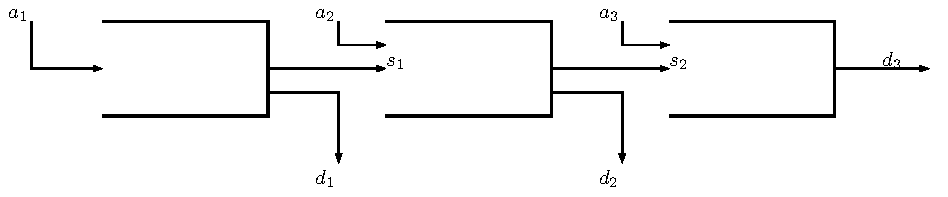
\includegraphics[scale=0.75]{tandem.pdf}
 \caption{A system with 3 queues}
\end{figure}

\subsection{Multicore machine}

In this section, we present the results of our simulation on a multicore machine.
This is close to the PRAM model we have presented since the communications cost between cores
are small and there is a large shared memory which can be used to write the trajectories as they are computed.

We made several practical optimizations to our algorithms: when the lower bound and the upper bound are computed in an interval,
we test whether there is a coupling. If we detect a coupling at step $T$ in the interval, we compute the real trajectory 
from this moment on and not the \emph{two bounds}. Moreover, we store the number $T$ so that the next time we simulate 
the interval, the simulation is stopped at $T$. Finally, we do not update $status_j$ to $\textsc{ToCompute}$ when it 
has already coupled and when the starting bounds $s_j^{min}$ and $s_j^{max}$ are different. Indeed, simulating the interval $j$
when it has already coupled will never help to compute other intervals.
 
To ensure that two cores do not write or read the status of an interval at the same time we need to use locks,
which can cause some performance penalties which are not visible when writing the ideal algorithm for a PRAM.
That is why we introduce a simple variant of \textsc{Speculative Sandwich} that we call \textsc{Fixed Interval}.
If we have $p$ cores available, then we set $t = n/p$ and each processor is affected to a specific interval. 
The algorithm is the following:  each processor simulates its interval and modify the bounds of the next and continue to do so until it has computed the right trajectory for its interval. This methods may waste time, in particular because we need to set
$t = n/p$ which means that as soon as the first interval is computed, a processor will go unused. On the other hand, it can be 
implemented without locks since each processor simulate a different part of the trajectory and that no status of the intervals must be maintained.


\todo{Dire ici la machine de test et mettre le résultat des expériences. Si on peut mettre en valeur les différences des algos le faire, en utilisant un temps de couplage moyen légérement plus grand que la taille d'un intervalle}


\subsection{Distributed computing}

In this section, we test our algorithms in a distributed computing settings. We use a master computer which dispatches
to several slave computers the simulation of the intervals according to the algorithm $\textsc{Speculative Sandwich}$.
It sends two states to a slave which are used as a starting point of the simulation. The master also maintains the status of each interval and of each slave (computing or not). When a simulation is finished the slave send back the two states obtained at the end 
to the master. This generates very little traffic on the network and the only problem is the latency: the time between the sending of a message and its reception may be long \todo{dire comme montré dans la figure blah}.  The only thing which has a large impact on the load of the network and may take more time than the simulation is the sending of the correct trajectory back to the master. Therefore we skip this part in our experiments. It is realistic, since most of the time the trajectory is not needed but rather statistics on it which can be transmitted much quicker. 

The master computer in our experiments is a MacBook Air and the slaves are $7$ Raspberry Pi $3$ (Model B) with $1GB$ of RAM. Note that the performances of the master are not relevant while the performances of the slaves directly impact the time to simulate a trajectory. The machines are connected to a local network through a $1$ $Gbs$ switch and communicate using sockets and the protocol TCP/IP. 


\todo{Pas besoin de faire une sous section, mais le but c'est de voir le cout d'un aller-retour par rapport à une étape de sim
pour bien régler la taille des intervalles}

Since our network uses a local network with TCP/IP, one must investigate the cost of the network in our simulations. 
In our source code, we fixed the size of a standard master/server message to 24 integers and the size of the server/master messages depends of the number of queues in the simulation. One must focus on the cost of sending a trajectory, which is by far the largest message, indeed, the size of a trajectory is equal to $t \times m$($t$ is the size of the interval, and $m$ is the number of queues). On the following experiment, we tried to compare the evolution of the cost of the computing time and the network cost for different number of queues going from 1 to 10. We arbitrary set the size of the interval $t$ to $10,000$, which is a good order of magnitude considering the following experiments. The points on fig|~\ref{fig:example} are some average times computed on 100 different simulations.

\begin{figure}[h]
\centering
 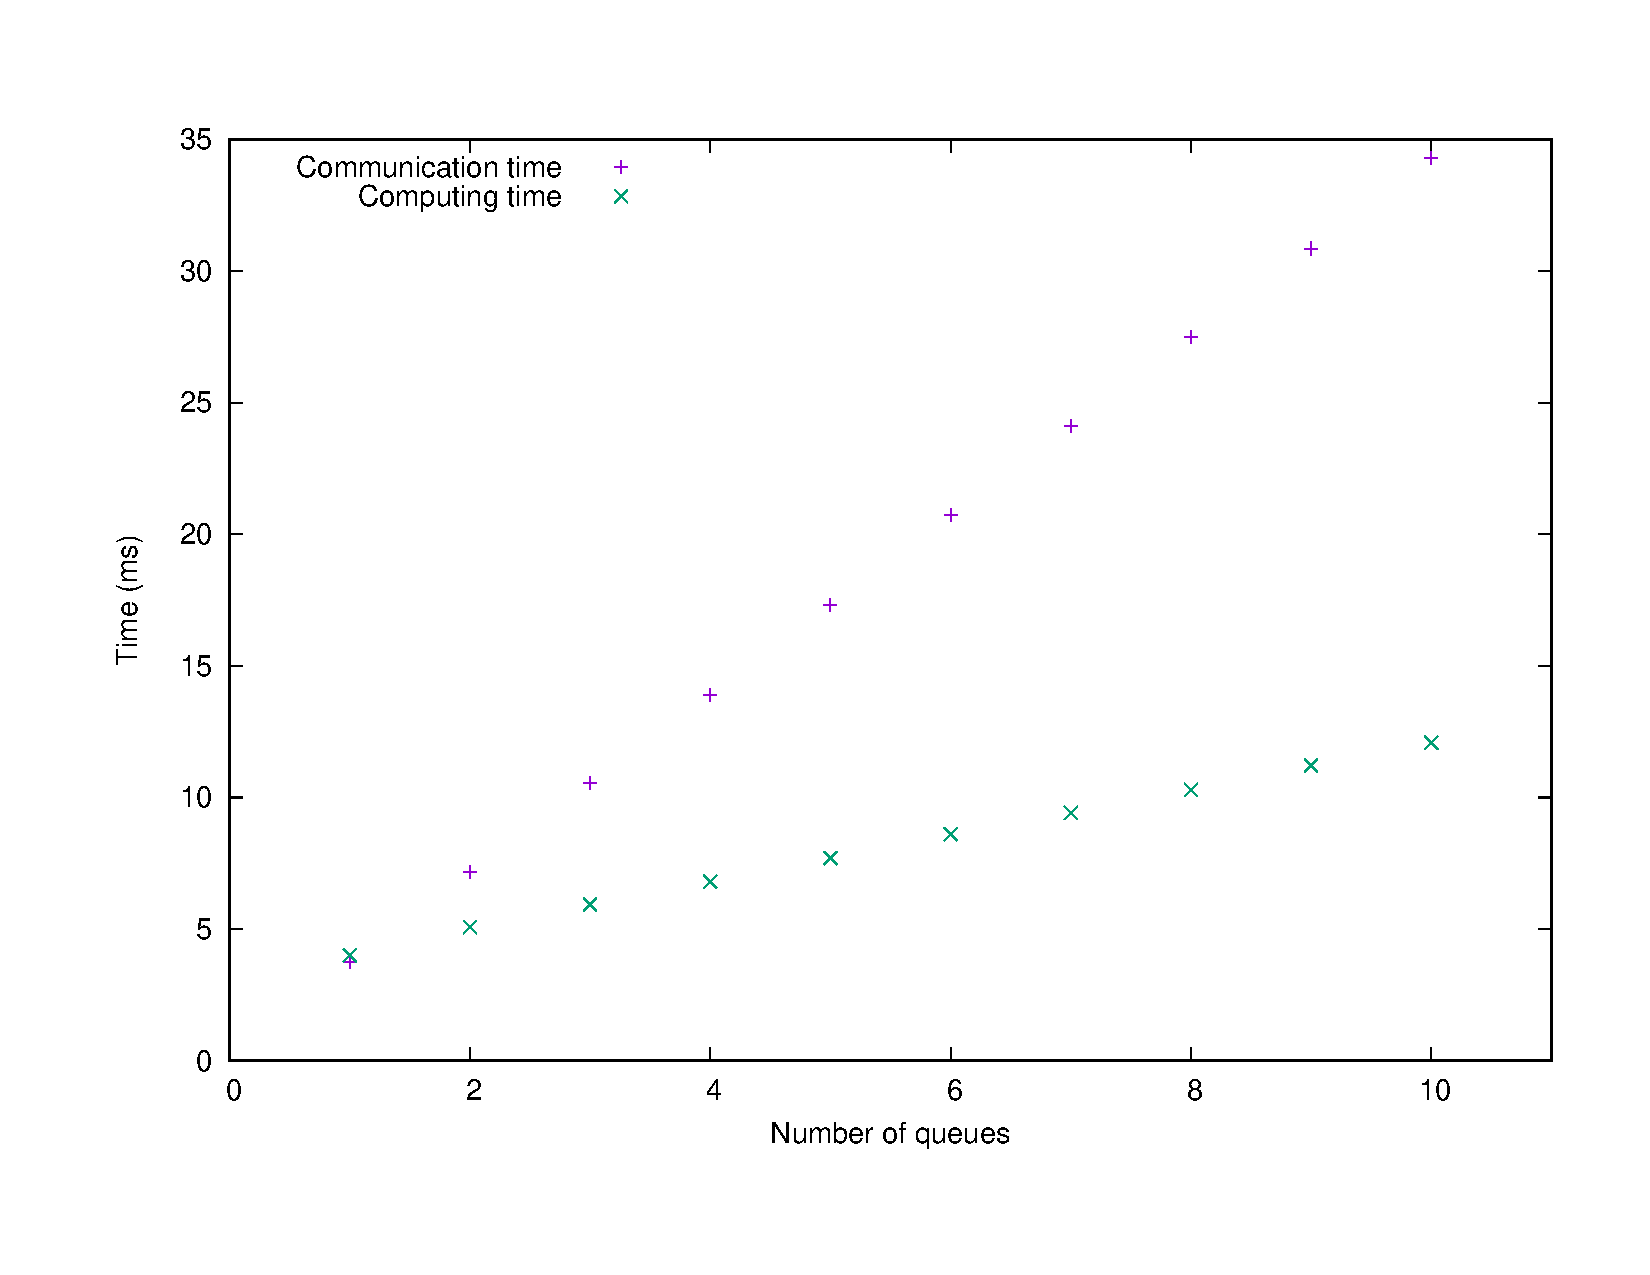
\includegraphics[scale=0.45]{time_traj.pdf}
 \caption{Evolution of the computing and communication time of a trajectory of $10,000$ events}
\end{figure}

As we can see, both the communication an computing times of a trajectory increases linerarly with the number of queues, but the communication time is increasing faster. A linear regression allowed us to calculate the slope of those two point clouds; the slope of the communication time is $3.390585$ while the slope of the computing time is only of $0.885585$. Both of those two correlations coefficients are greater $0.999$. Thus, to avoid an over domination of the network time, which would hide every interesting results, in the following experiments, we will consider a little number of queues in tandem.

\subsection{Algorithm performance evaluation}
We now want to measure the performance of the \textsc{Smallest Parallel Sandwich} and the \textsc{Balanced Parallel Sandwich}, compared to the One bound algorithm (cf sec~\ref{sec:onebound}). In the following experiment we thus take a random process with $5$ queues, which allows us to have a reasonable amount of computation in the servers, and a not too high $\frac{ \textrm{Network time} }{\textrm{Computing time}}$ ratio. In order to choose the size $n$ of the simulation, we made an upstream experiment to determine the average time between the coupling of the two bounds, for two queues, with the parameters we give in sec~\ref{sec:randomproc}. Thus, this average coupling time is to $28,049$, calculated over $100$ simulations.

\subsubsection{Long simulation}
We first want to look at the behavior of our algorithms in a simulation in which there is an high probability to have a coupling during the computing of a single interval. We then set the size of the simulation to $n = 210,000$. Fig.~\ref{fig:interslong} and ~\ref{fig:timelong} show the results of respectively, the average sum of the lengths of the intervals computed, and the average total time if simulation in regard of the number of intervals, over $100$ instances. By the way, the size of the interval directly depends of the number of intervals. The total size of the simulation is always the same, that is, $210,000$. We used $7$ servers in those experiments.

\begin{figure}[H]
\centering
\label{fig:interslong}
 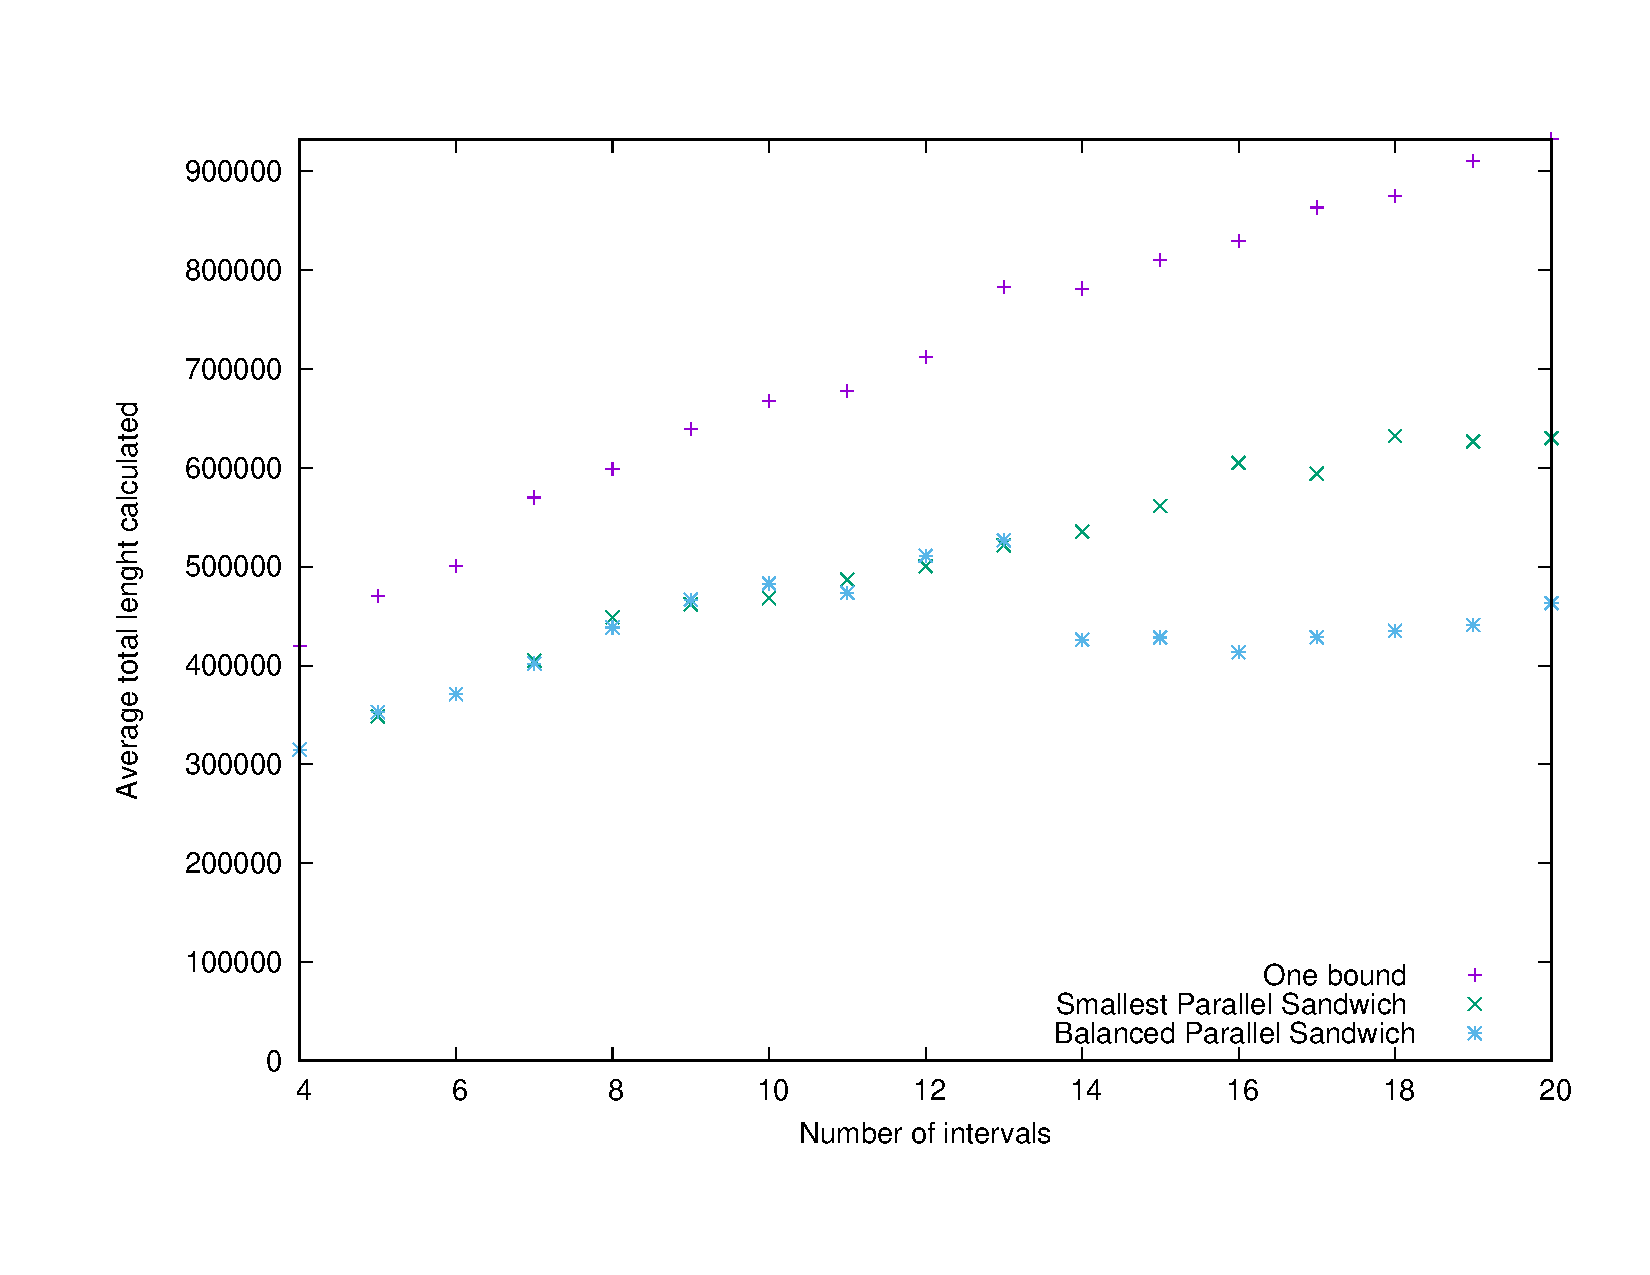
\includegraphics[scale=0.45]{interslong.pdf}
 \caption{Evolution of the average of the sum of the lengths of the intervals computed for $100$ simulations of $210,000$ events.}
\end{figure}

\begin{figure}[H]
\centering
\label{fig:timelong}
 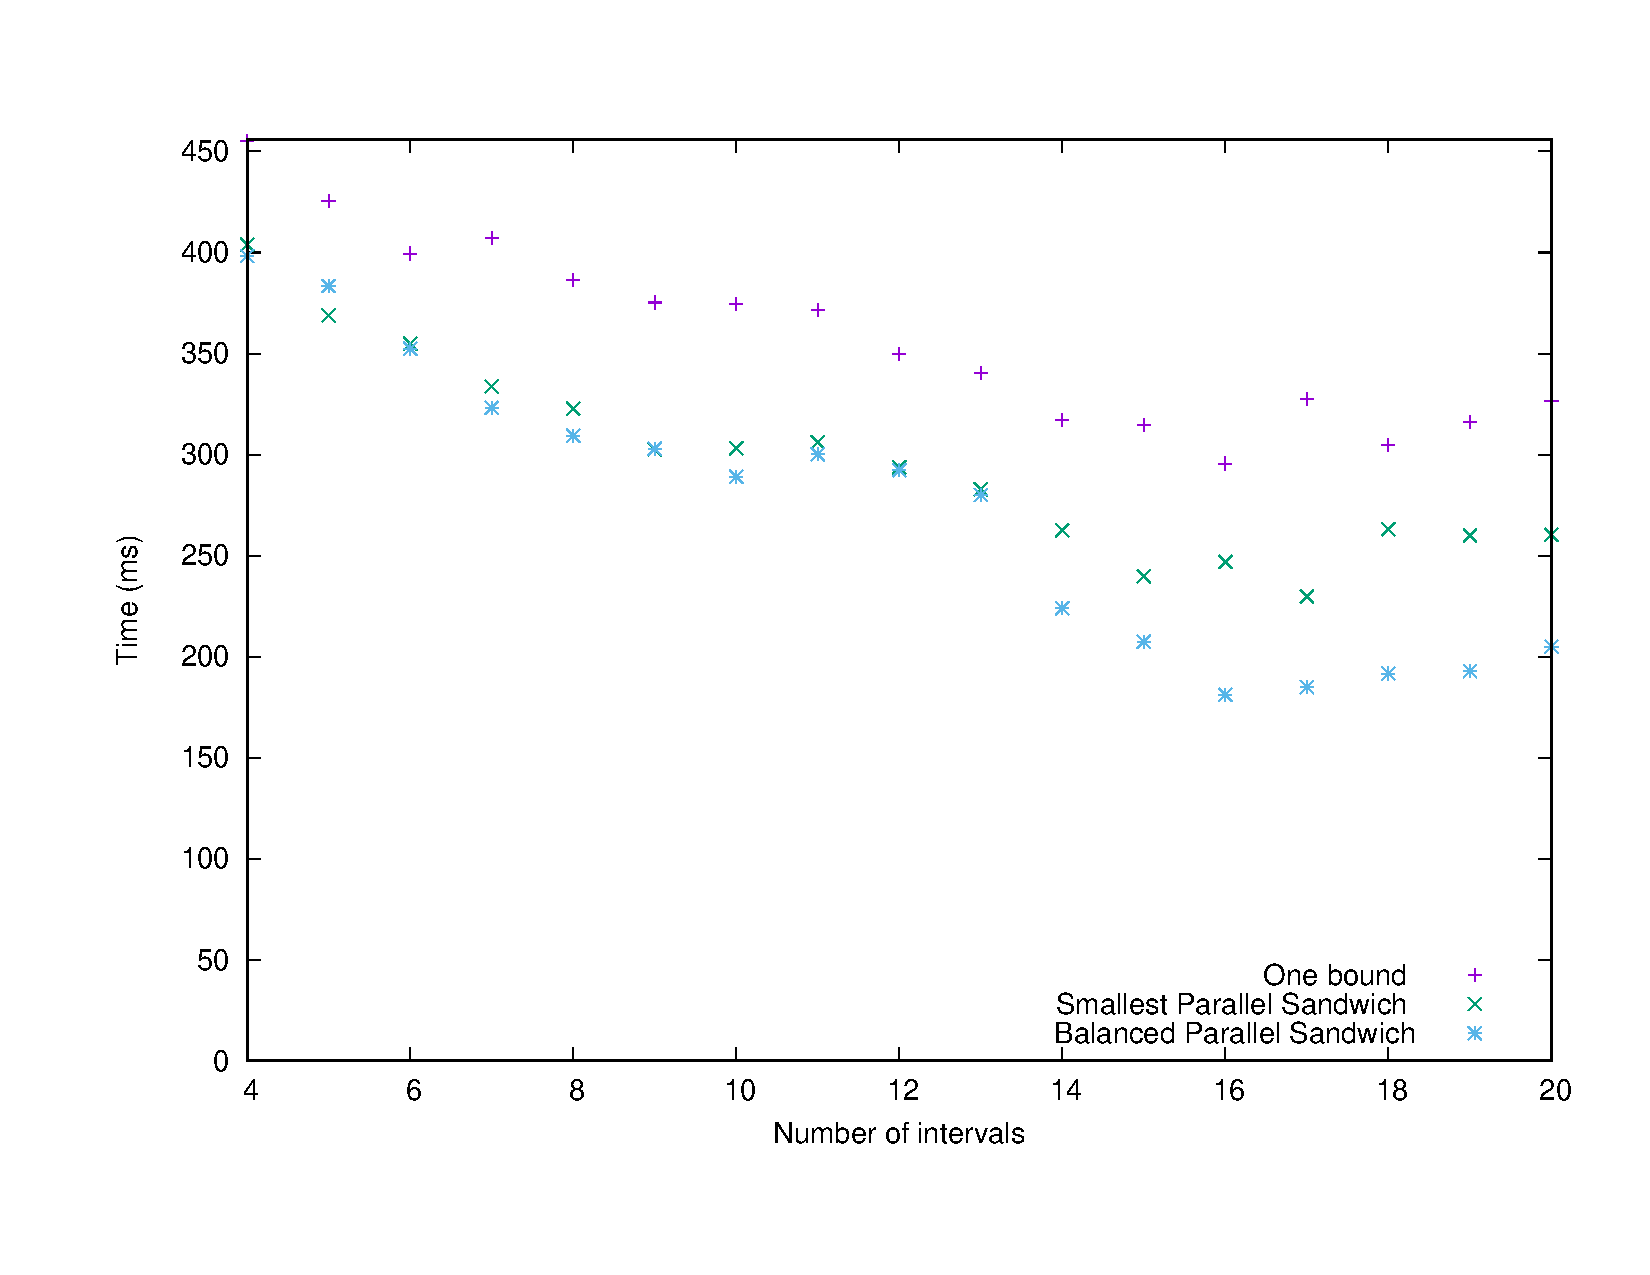
\includegraphics[scale=0.45]{timelong.pdf}
 \caption{Evolution of average for $100$ simulations of $210,000$ events.}
\end{figure}


First, we remark that the \textsc{Smallest Parallel Sandwich}  and the \textsc{Balanced Parallel Sandwich} are always better than the One Bound algorithm. The weak increasing trend for One Bound and \textsc{Smallest Parallel Sandwich} on fig.~\ref{fig:interslong} might be due to the decreasing probability of coupling in one interval when the number of intervals increases. Nevertheless the \textsc{Balanced Parallel Sandwich} seems to have a different behavior after an undetermined threshold. We will study this phenomenon later.

\todo{pas vraiment en fait, j'utilise le fait que il y ait ce point du rupture pour comparer les performances en fonction du nombre de servers mais je ne sais pas du tout pourquoi ca fait ca??}

In contrast to those results, as we can see on fig.~\ref{fig:timelong} , it looks like having few long intervals is more expensive in time than having more shorter intervals. This might be due to the network. Indeed, as we observed in the results of sec.~\ref{sec:networkimpact}, the more the interval is long, the more network increases. Moreover, the experiment in sec.~\ref{sec:networkimpact} were made on a single server communicating with the master. Here, we have 7 servers which probably create some contention, and thus, some additional latency.
On a single processor, the average time on $100$ simulations for $210,000$ events is to $162.13$ ms.

To make sure that the network is dominating the simulation time, we investigate the activity of the servers during the experiments. Fig.~\ref{fig:servers} shows the average repartition of the computation, network and waiting time of the servers, during the previous experiments, for the computation of the \textsc{Balanced Parallel Sandwich} simulations.


\begin{figure}[H]
\centering
\label{fig:servers}
 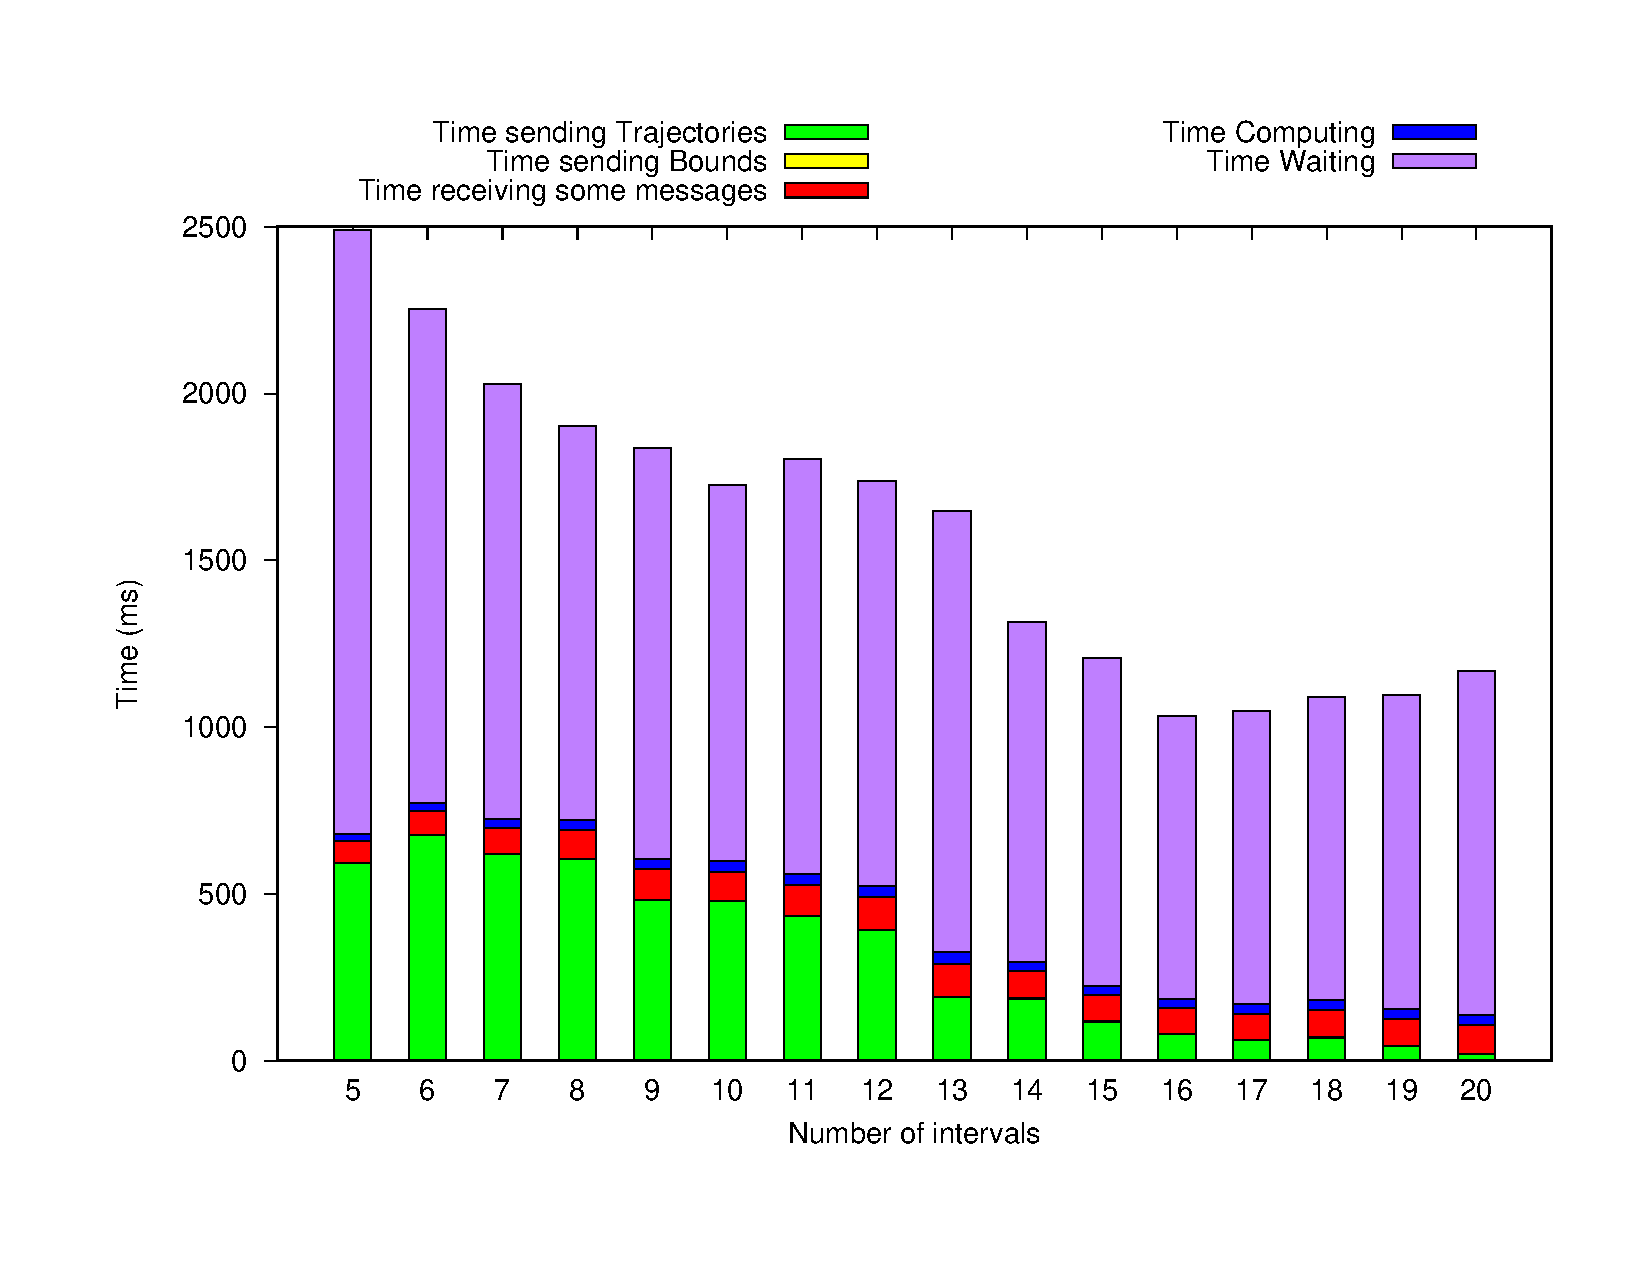
\includegraphics[scale=0.45]{server.pdf}
 \caption{Repartition of the activities of the processors during the simulation.}
\end{figure}

First, we can see that, the most of the time, the servers are waiting for something to do. Since the master algorithm is not very complicated, we suppose that the network highly slows the communication between the master and the servers. The rest of the time, the servers are mainly computing some network operations (sending, receiving).
\subsubsection{Short simulation}
We then tried to look if there is a difference when the simulation is short. The following experiment are made with exactly the same parameters than upward, except the simulation length, which is now of $30,000$. In this situation, the probability of coupling is very low.

\begin{figure}[H]
\centering
\label{fig:intersshort}
 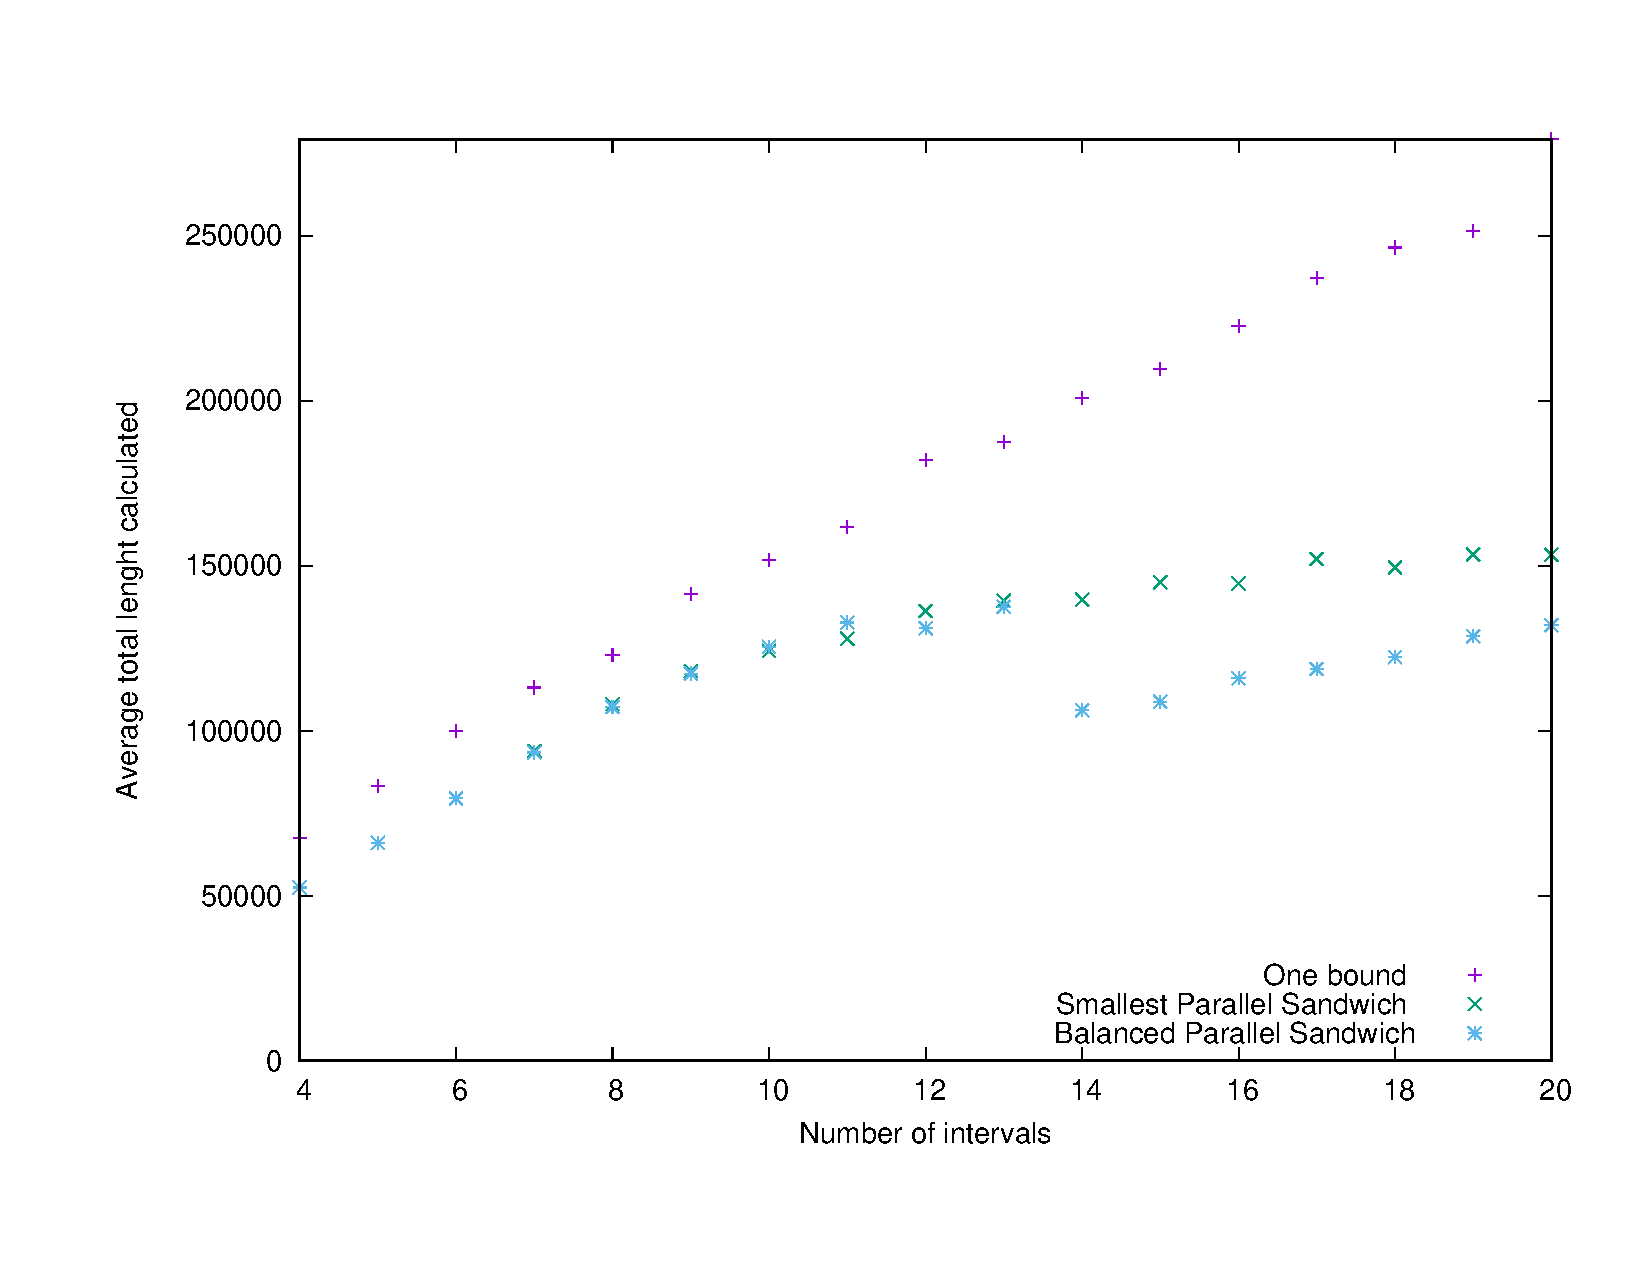
\includegraphics[scale=0.45]{intersshort.pdf}
 \caption{Evolution of the average of the sum of the lengths of the intervals computed for $100$ simulations of $30,000$ events.}
\end{figure}

\begin{figure}[H]
\centering
\label{fig:timeshort}
 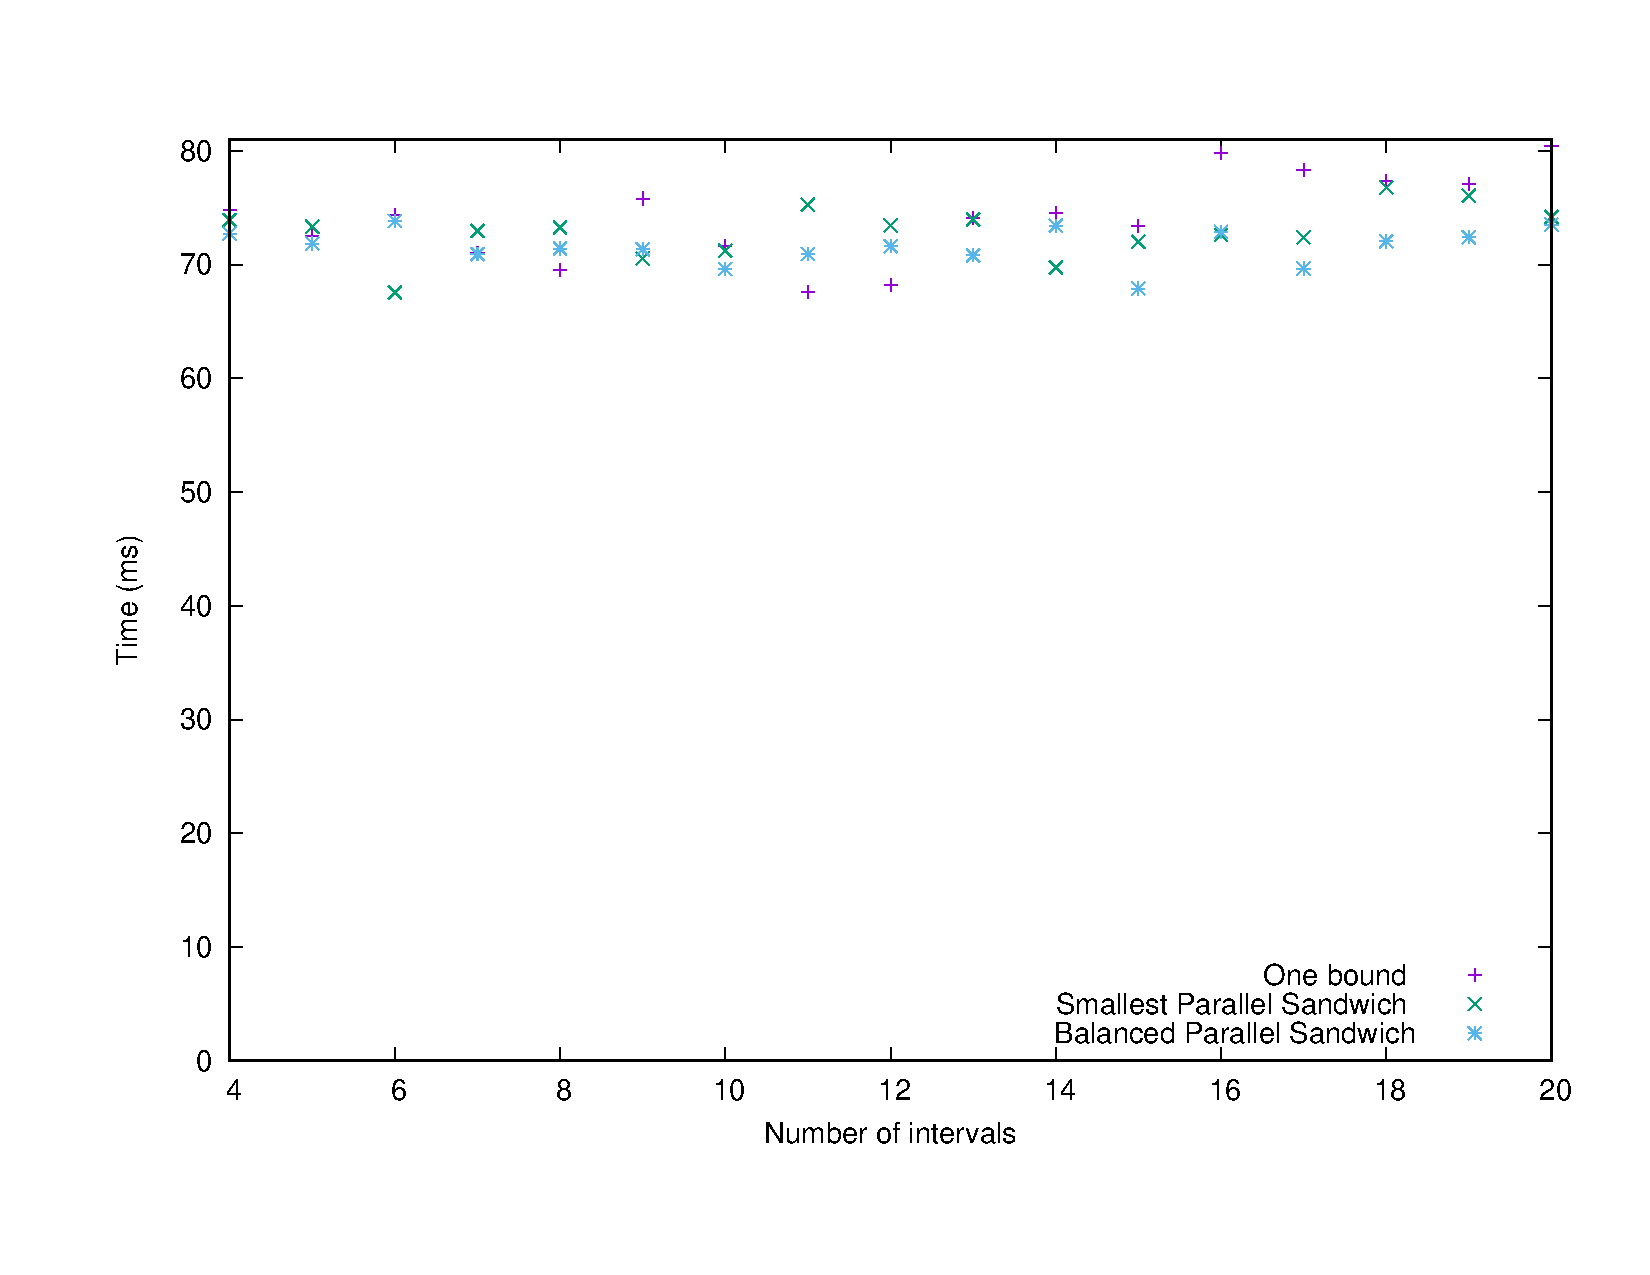
\includegraphics[scale=0.45]{timeshort.pdf}
 \caption{Evolution of average for $100$ simulations of $30,000$ events.}
\end{figure}

The trend of the curves on fig.~\ref{fig:intersshort} are notably similar to the curves of fig.~\ref{fig:interslong}. 
On the other hand, the three algorithm seems to run in a similar time on fig.~\ref{fig:timeshort}. Once again, this is due to the domination of the network time, which is the same for all algorithms, since the messages are all short.
On a single processor, the average time on $100$ simulations for $30,000$ events is to $23.06$ ms.
\todo{expliquer un peu plus, de toute facon on calcule tout les intervals en attendant le gars du debut vu que ca a tres peu de chance de coupler}

=======

\todo{Dire ce qui est utilisé comme techno entre les raspberry et donc la latence induite (à mesurer)}
>>>>>>> 43f1c719ccab17cdd0288dfaf16a9cd2cea56835

\subsection{Number of server used}
We now want to study the impact of the number of server used. As we noticed in fig.~\ref{fig:interslong}, there is an interessant point when the number of intervals is twice the number of servers (this threshold was observed for any number of servers between 2 and 7). We then look at the execution time of $100$ simulation from $2$ to $7$ servers, whith the \textsc{Balanced Parallel Sandwich} algorithm. The number of event $n$ of the simulation is set to $210,000$, and the number of intervals is always set to $2 \times \textrm{number of servers}$, since it is the first number at which the execution time of the algorithm starts to stagnate to it's lower value, for any number of processors.

\begin{figure}[H]
\centering
\label{fig:nbservs}
 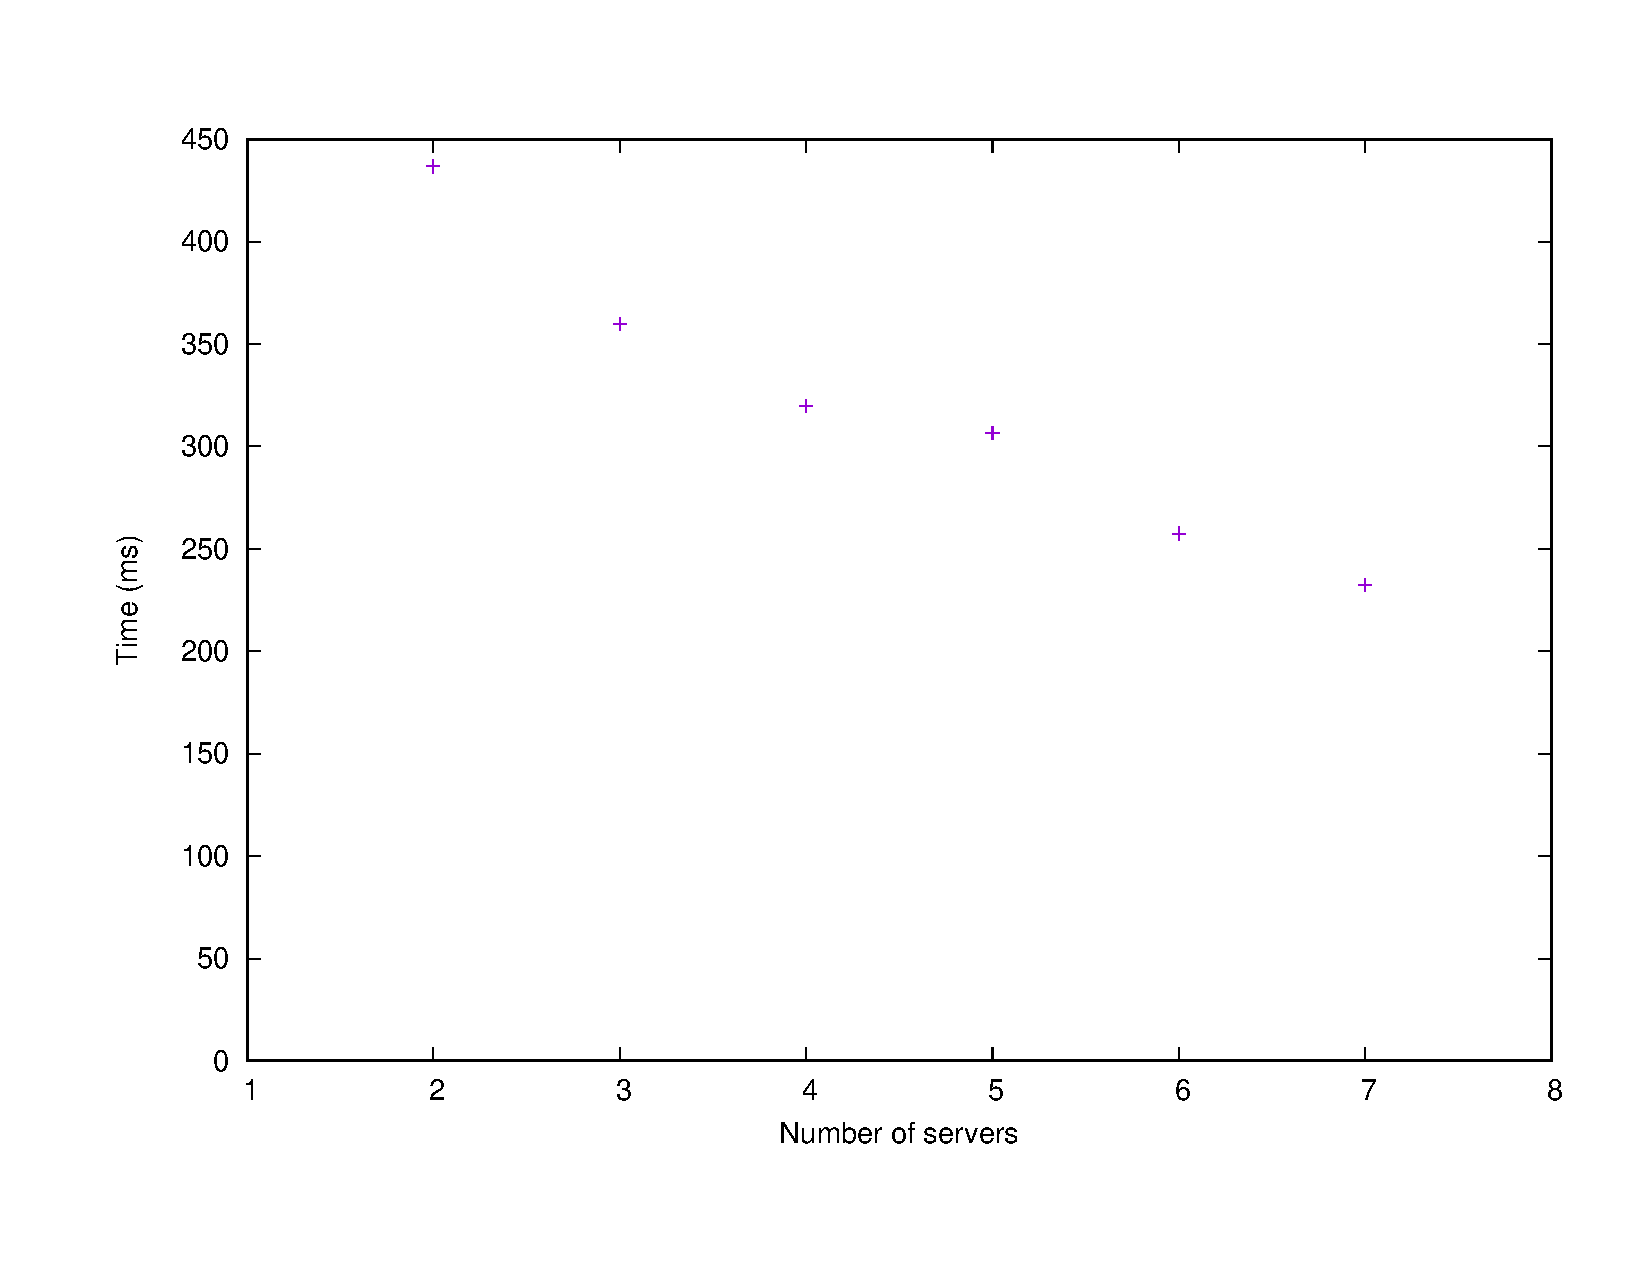
\includegraphics[scale=0.45]{numberofservers.pdf}
 \caption{Impact of the number of servers on the execution time.}
\end{figure}

As we can see on fig.\ref{fig:nbservs}, the more we have servers, the faster the algorithm runs.
\todo{bof cette conclusion, vu que c'est le reseau qui masque tout}

Practical problems: cost of the network transmission, especially for transmitting long sequences.
-> measure the time of a two way trip for a small message and the time of sending an interval.
To say that in practice we will not compute the whole sequence but statistic on it which could help
reduce the use of the network.


\bibliographystyle{plain}
\bibliography{biblio.bib}

\end{document}
